    \newcommand{\sizeS}{.125}
    \newcommand{\sizeP}{.125}
    \newcommand{\hh}{.175\textwidth}
    \newcommand{\ww}{.200\textwidth}
    \setlength{\tabcolsep}{.5pt}
    \centering
    \tiny
    %\setlength{\tabcolsep}{2pt}
    \begin{tabular}{c|c|c|c|c|c|c|c}
        & Input image &  Grad-CAM  & Grad-CAM++ & Score-CAM & Ablation-CAM & XGrad-CAM & Opti-CAM 
     \\
    
        \rotatebox{90}{\tiny~Grass Snake} &
        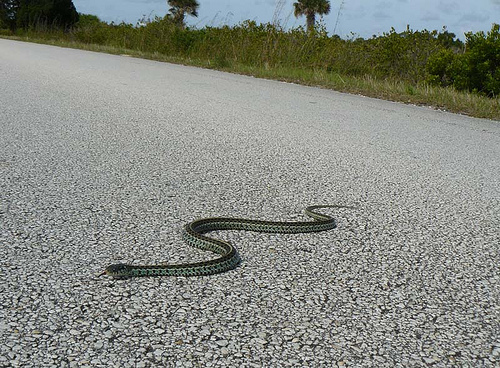
\includegraphics[trim={36mm 10mm 32mm 10mm},clip, width=\sizeP\textwidth]{fig/opticam/mainfig/img/select/ILSVRC2012_val_00000006.JPEG}&
        \fig[\sizeS]{opticam/mainfig/img/select/ILSVRC2012_val_00000006JPEG_vgg_GradCAM_vis.png} &
        \fig[\sizeS]{opticam/mainfig/img/select/ILSVRC2012_val_00000006JPEG_vgg_GradCAMPlusPlus_vis.png} &
        \fig[\sizeS]{opticam/mainfig/img/select/ILSVRC2012_val_00000006JPEG_vgg_ScoreCAM_vis.png} &
        \fig[\sizeS]{opticam/mainfig/img/select/ILSVRC2012_val_00000006JPEG_vgg_AblationCAM_vis.png} &
        \fig[\sizeS]{opticam/mainfig/img/select/ILSVRC2012_val_00000006JPEG_vgg_XGradCAM_vis.png} &
        \fig[\sizeS]{opticam/mainfig/img/select/ILSVRC2012_val_00000006JPEG_vgg_versionP0_vis.png}  \\
    
        \rotatebox{90}{\tiny~Tricycle} &
        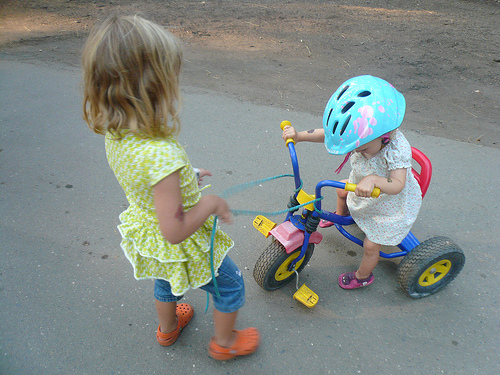
\includegraphics[trim={28mm 10mm 39mm 10mm},clip, width=\sizeP\textwidth]{fig/opticam/mainfig/img/select/ILSVRC2012_val_00000069.JPEG}&
        \fig[\sizeS]{opticam/mainfig/img/select/ILSVRC2012_val_00000069JPEG_vgg_GradCAM_vis.png} &
        \fig[\sizeS]{opticam/mainfig/img/select/ILSVRC2012_val_00000069JPEG_vgg_GradCAMPlusPlus_vis.png} &
        \fig[\sizeS]{opticam/mainfig/img/select/ILSVRC2012_val_00000069JPEG_vgg_ScoreCAM_vis.png} &
        \fig[\sizeS]{opticam/mainfig/img/select/ILSVRC2012_val_00000069JPEG_vgg_AblationCAM_vis.png} &
        \fig[\sizeS]{opticam/mainfig/img/select/ILSVRC2012_val_00000069JPEG_vgg_XGradCAM_vis.png} &
        \fig[\sizeS]{opticam/mainfig/img/select/ILSVRC2012_val_00000069JPEG_vgg_versionP0_vis.png}  \\

        %\rotatebox{90}{~Komondor} &
        %\fig[\sizeS]{opticam/mainfig/img/visual/ILSVRC2012_val_00001113.png}&
        %\fig[\sizeS]{opticam/mainfig/img/visual/Resnet50_GradCAM_ILSVRC2012_val_00001113.png} &
        %\fig[\sizeS]{opticam/mainfig/img/visual/Resnet50_GradCAMPlusPlus_ILSVRC2012_val_00001113.png} &
        %\fig[\sizeS]{opticam/mainfig/img/visual/Resnet50_ScoreCAM_ILSVRC2012_val_00001113.png} &
        %\fig[\sizeS]{opticam/mainfig/img/visual/Resnet50_AblationCAM_ILSVRC2012_val_00001113.png} &
        %\fig[\sizeS]{opticam/mainfig/img/visual/Resnet50_XGradCAM_ILSVRC2012_val_00001113.png} & 
        %\fig[\sizeS]{opticam/mainfig/img/visual/Resnet50_OptCAM_ILSVRC2012_val_00001113.png}  \\\pause
            
        \rotatebox{90}{\tiny~Pneumonia} &
        \fig[\sizeS]{opticam/mainfig/img/medical/chest_VGG16_GradCAM_1_img.png} &
        \fig[\sizeS]{opticam/mainfig/img/medical/chest_VGG16_GradCAM_1_vis.png} &
        \fig[\sizeS]{opticam/mainfig/img/medical/chest_VGG16_GradCAMPlusPlus_1_vis.png} &
        \fig[\sizeS]{opticam/mainfig/img/medical/chest_VGG16_ScoreCAM_1_vis.png} &
        \fig[\sizeS]{opticam/mainfig/img/medical/chest_VGG16_AblationCAM_1_vis.png} &
        \fig[\sizeS]{opticam/mainfig/img/medical/chest_VGG16_XGradCAM_1_vis.png} &
        \fig[\sizeS]{opticam/mainfig/img/medical/chest_VGG16_OptCAM_plain_1_vis.png}  \\\pause
    
    
        \rotatebox{90}{\tiny~Pylorus} &
        \fig[\sizeS]{opticam/mainfig/img/medical/kvasir_Resnet50_GradCAM_3_img.png} &
        \fig[\sizeS]{opticam/mainfig/img/medical/kvasir_VGG16_GradCAM_3_vis.png} &
        \fig[\sizeS]{opticam/mainfig/img/medical/kvasir_VGG16_GradCAMPlusPlus_3_vis.png} &
        \fig[\sizeS]{opticam/mainfig/img/medical/kvasir_VGG16_ScoreCAM_3_vis.png} &
        \fig[\sizeS]{opticam/mainfig/img/medical/kvasir_VGG16_AblationCAM_3_vis.png} &
        \fig[\sizeS]{opticam/mainfig/img/medical/kvasir_VGG16_XGradCAM_3_vis.png} &
        \fig[\sizeS]{opticam/mainfig/img/medical/kvasir_VGG16_OptCAM_plain_3_vis.png}  \\
    
    \end{tabular}
